
\chapter{Osnovni pojmovi} % Main chapter title


%------------------------------------------------------------------------------

Svi živi organizmi sastoje se od jedne ili više ćelija, a svaka ćelija od
molekula. Veliki\footnote{ Obično se molekulska masa od $1000 Da$ (Daltona) uzima kao 
granica između malih molekula i makromolekula.}
molekuli (makromolekuli) organskog porekla obično\footnote{
  Lipidi recimo nisu polimeri, ali su principijalno slični
} su sačinjeni od
ponavljajućih strukturnih jedinica \keyword{monomera} \textit{(mono- = jedan,
mer- = deo)} međusobno povezanih \keyword{kovalentnim} vezama.  Takav molekul
zovemo \keyword{polimer} \textit{(poli- =mnogo, -mer= deo)}. 
% Polimer može da bude \textit{homo-polimer}, sačinjen od jednog tipa monomera
% ili suprotno \textit{hetero-polimer}, sačinjen od nekoliko raznih tipova
% monomera.
Skup monomera možemo da smatramo azbukom koja gradi jezik polimera.  Mali broj
monomera je dovoljan za strukturnu kompleksnost bilo koje ćelije.  Tri 
najznačajnija tipa bioloških polimera i njihovi monomeri prikazani su u Tabeli
\ref{tab:polimeri}.

\begin{table}[htpb]
  \centering
  \caption{Najznačajniji biološki polimeri}
  \label{tab:polimeri}
  \begin{tabular}{|l|l|}
    \hline
    \keyword{Polimer}            & \keyword{Monomer} \\
    \hline
    Ugljeni hidrati              & Monosaharid (šećeri) \\
    Nukleinska kiselina (DNK)    & Nukleotid \\
    Protein                      & Aminokiselina \\
    \hline
  \end{tabular}
\end{table}


\section{Centralna dogma molekularne biologije}

Centralna dogma molekularne biologije prikazana Slikom \ref{fig:dogma}
objašnjava protok informacija kroz generacije i ćeliju.

\begin{figure}[th]
\centering
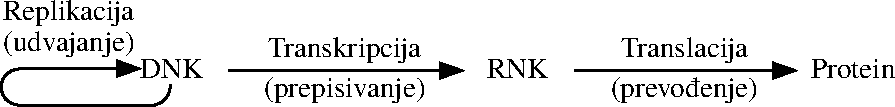
\includegraphics[]{uvod/centralna_dogma}
\caption { Centralna dogma molekularne biologije }
\label{fig:dogma}
\end{figure}


Dezoksiribonukleinska kiselina, kraće \keyword{DNK} se procesom replikacije
(tokom deobe ćelije) udvaja u dve kopije. Za života ćelije, regioni DNK
molekula tzv. \keyword{geni} bivaju transkribovani (prepisani) u oblik
ribonukleinske kiseline, kraće \keyword{RNK}. Glasnička RNK, kraće \keyword{mRNK}
dobijena transkripcijom tzv. \keyword{kodirajućeg gena} sadrži kodirane informacije
za sintezu proteina i biva transportovana do molekulskih mašina ribozoma.
Ribozom dekodira poruku mRNK odnosno translira (prevodi) mRNK  u protein.
Pomenuti kod prikazan centralnim delom Slike \ref{fig:kod} zove se
\keyword{genetički kod} i opisuje mapiranje uzastopnih trojki baza nukleinske
kiseline tzv. \keyword{kodona} u aminokiseline ili stop oznaku. Na primer,
trojka baza: guanin-adenin-uracil (GAU) ili guanin-adenin-citozin (GAC) prevode
su u asparginsku kiselinu.

\begin{figure}[]
\centering
\hspace*{-2.3cm} 
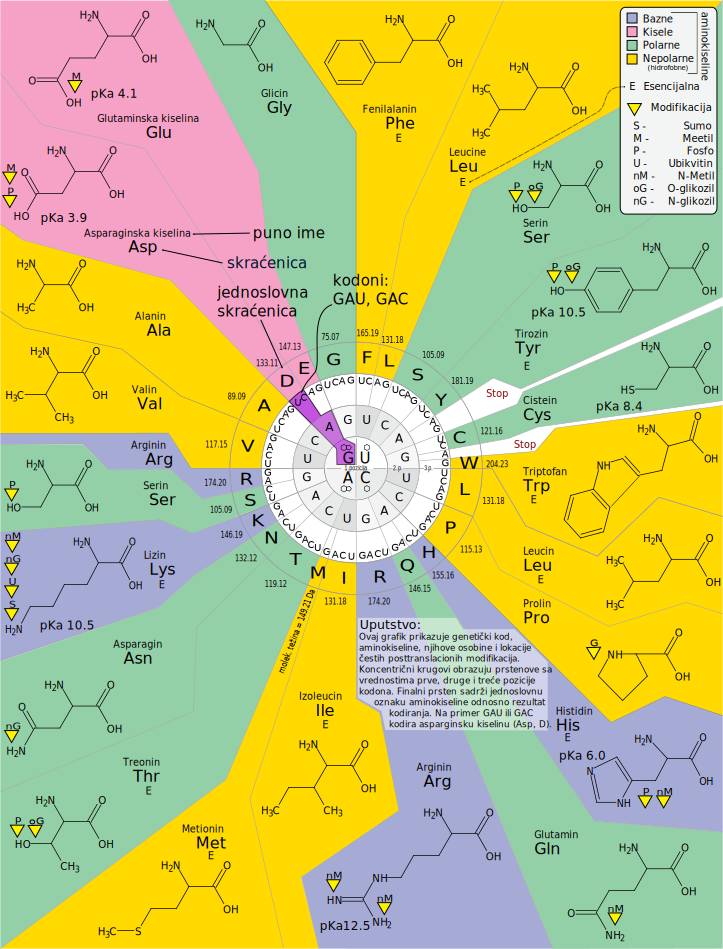
\includegraphics[scale=0.94]{uvod/geneticcode}
\caption { Genetički kod, aminokiseline, osobine AK i lokacije PTM\\
  \footnotesize
(Originalna Slika pripada vikimedija javnom domenu, autor Bromomir)}
\label{fig:kod}
\end{figure}

\clearpage

Genetički kod smatra se univerzalnim za sva živa bića (poznat kao kanonski).
Ipak, sitne razlike u tumačenju nekih kodona javljaju se kod malog broja vrsta,
obično nekih arhea, bakterija ali i mitohondrija.

\keyword{Gen} je region DNK sekvence
koji biva transkribovana u RNK.  Neki geni su tzv.  \keyword{nekodirajući geni} i
transkribuju se u funkcionalne RNK molekule dok gore pomenuti \keyword{kodirajući geni}
služe sintezi proteina.  Proces prepisivanja gena u funkcionalnu jedinicu još
se naziva \keyword{ekspresija gena}, a rezultat \keyword{genski produkt}.
Kompletan DNK kod nekog organizma predstavlja njegov
\keyword{genom}, dok  svi transkribovani RNK molekuli čine \keyword{transkriptom},
a svi sintetisani proteini \keyword{proteom}.  Tri velike oblasti
bioinformatike koje prikupljaju i analiziraju ove podatke su:
\keyword{genomika}, \keyword{transkriptomika} i \keyword{proteomika}.
U bioinformatici gene i genske produkte najjednostavnije predstavljamo
sekvencama njihovih respektivnih monomera.


Centralnu dogmu predložio je Frensis Krik 1958. godine. Ipak, vremenom 
razni specijalni slučajevi toka informacija su otkriveni, prvenstveno kod
virusa i bakterija. U ovom radu nećemo ih razmatrati.

\section{Homologija}

Dve sekvence su \keyword{homologe} ako dele zajedničkog evolutivnog pretka
(originalna sekvenca). Skup homologih proteina čine \keyword{proteinsku
familiju}. Homologi proteini skoro uvek dele sličan trodimenzionalan oblik.
Međutim, isto se ne može reći za sličnost samih sekvenci jer sadržaj sekvence
brže divergira od oblika koji kodira. Razlikujemo dva tipa homologa:
\begin{itemize}
  \item
    Dve sekvence su \keyword{ortologe} (orto - pravi) ako predstavljaju istu
    sekvencu (isti gen, protein) u različitim vrstama nastalu specijalizacijom.
    Na primer, geni mioglobina kod čoveka i kod pacova su ortolozi. Ortolozi
    uvek obavljaju istu funkciju u ćeliji.

  \item Dve sekvence su \keyword{paraloge} ako su nastale duplikacijom
    originalne sekvence. U slučaju duplikacije, jedna sekvenca može
    da se promeni i služi različitoj funkciji. Na primer, ljudski
    alfa globin i beta globin su paralozi.
\end{itemize}

Pošto je tačan trodimenzionalan oblik retko poznat, pronalaženje homologa
se oslanja na sličnost sekvenci. Postoje razne metode za poređenje
(poravnanje) sekvenci od kojih se za pronalaženje homologa najčešće koriste
PSI-BLAST (ili noviji, senzitivniji DELTA-BLAST).  PSI-BLAST \en{
position-specific iterated BLAST, $\psi$-BLAST } prvo gradi PSSM matricu
originalne sekvence (od bliskih, sličnih sekvenci) koju dalje koristi u pretrazi
udaljenih proteinskih sekvenci. PSSM \en{Position-Specific Scoring Matrix} je
$20 \times n$ matrica koja sadrži verovatnoću pojavljivanja aminokiselina
za svaku od $n$ pozicija sekvence. PSSM se generiše iz poravnanja nekoliko
sličnih sekvenci. Rezultat pretrage može se agregirati u novu PSSM koja
predstavlja evolutivni profil i opisuje familiju proteina. 

\label{sec:}
\section{Proteini}

Proteini (belančevine) su najčešći biološki makromolekuli koji čine i do $80\%$
suve mase organizma.  Strukturno, protein je linearan polimer sačinjen od lanca
\keyword{aminokiselina} (monomeri) skraćeno AK.

\subsection{Aminokiseline}
Aminokiseline koje translacijom mRNK ulaze u sastav proteina poznate su kao
\keyword{proteinogene}\footnote{U prirodi se javljaju stotine različitih AK, ali
one ne ulaze u sastav proteina}.  Do danas, otkrivene su 22 proteinogene
aminokiseline od kojih je 20 kodirano kanonskim genetičkim kodom tzv.
\keyword{standardne} AK, dok se 21. AK (selenocistein) i 22. AK (pirolizin)
prevode specijalnim tumačenjem STOP kodona i to samo kod nekih organizama\footnote{
  selenocistein se javlja u svim domenima života (arhea, bakterija i
  eukariota), ali ne i kod svih vrsta organizama, dok se pirolizin javlja samo
kod određenih bakterija i arhea}. 

Proteinogene aminokiseline imaju šablon strukturu predstavljenu Slikom \ref{fig:AK} a).
Centralni alfa ugljenikov atom ($C_{\alpha}$) povezan je \keyword{amino grupom} ($-NH_2$), 
\keyword{karboksilnom grupom} ($-COOH$), atomom vodonika i tzv. \keyword{R grupom}.
Vrsta aminokiseline određena je R grupom još poznatom kao \keyword{bočni niz} ili \keyword{bočni ostatak} \en{residue}.

Reakcijom kondenzacije prikazane na Slici \ref{fig:AK}b dve aminokiseline grade
kovalentnu tzv. peptidnu vezu rezultujući peptidom (dipeptid na slici).  Dakle,
peptid je polimer aminokiselina koje su međusobno povezane peptidnim vezama.
Peptid duži od 10 AK (Slika \ref{fig:AK}c ) se smatra polipeptidom (skraćeno
pp). Pod proteinom se podrazumeva polipeptid velike dužine. Različiti izvori
navode različite granice, na primer: 20-30 AK, 50 AK ili 100 AK, ali zapravo ne
postoji jasna granica između polipeptida i proteina
\parencite{protein_slajdovi}. Ponavljajući elementi $N-C_\alpha-C$
$(-N-C_\alpha-C)^*$ $-N-C_\alpha-C$ čine tzv.  \keyword{pp lanac} ili
\keyword{kičmu peptida} sa koje štrče bočni nizovi.  Polipeptidi se zapisuju u
smeru u kome su sintetisani pa zato  početak (levi kraj) nazivamo N-terminus
(zbog amino grupe), a desni kraj C-terminus (zbog
karboksilne grupe).


Prema fizičkim i hemijskim osobinama bočnog niza, aminokiseline se mogu
klasifikovati na nekoliko načina prikazanih Slikama \ref{fig:kod} i
\ref{fig:AK_vene} od čega izdvajamo sledeću klasifikaciju:
\begin{itemize}
  \item Nepolarne AK -
    zbog manjka asimetrije u naelektrisanju R grupe ovi molekuli nisu
    rastvorljivi u vodi (koja je polaran molekul). Hidrofobni su (ne vole
    vodu).  Obično se ove aminokiseline nalaze u unutrašnjosti savijenog proteina gde
    je kontakt sa vodom mimimalan.
    
  \item Nenaelektrisane polarne AK -
    rastvorljive u vodi (vole vodu). Uglavnom se nalaze na spoljnim
    delovima proteina, često na hemijski aktivnim delovima.

  \item Naelektrisane polarne AK -
    veoma hidrofilne. Dodatno se dele na pozitivno i negativno naelektrisane.

  \item Aromatične AK - najveće i najtežim jer u bočnom nizu sadrže 
    aromatični prsten (jedan ili više) od ugljenikovih atoma.
\end{itemize}

Za vreme života proteina (nakon translacije) aminokiseline koje ga čine mogu
biti modifikovane od strane raznih enzima, na primer pravljenjem kovalentnih
veza sa novim funkcionalnim grupama. Ovaj proces poznat je kao
\keyword{posttranslaciona modifikacija}, kraće \keyword{PTM}.  Na Slici
\ref{fig:kod} prikazane su najčešće PTM i gde se javljaju.

\begin{figure}[th]
\centering
% \hspace*{-2.0cm} 
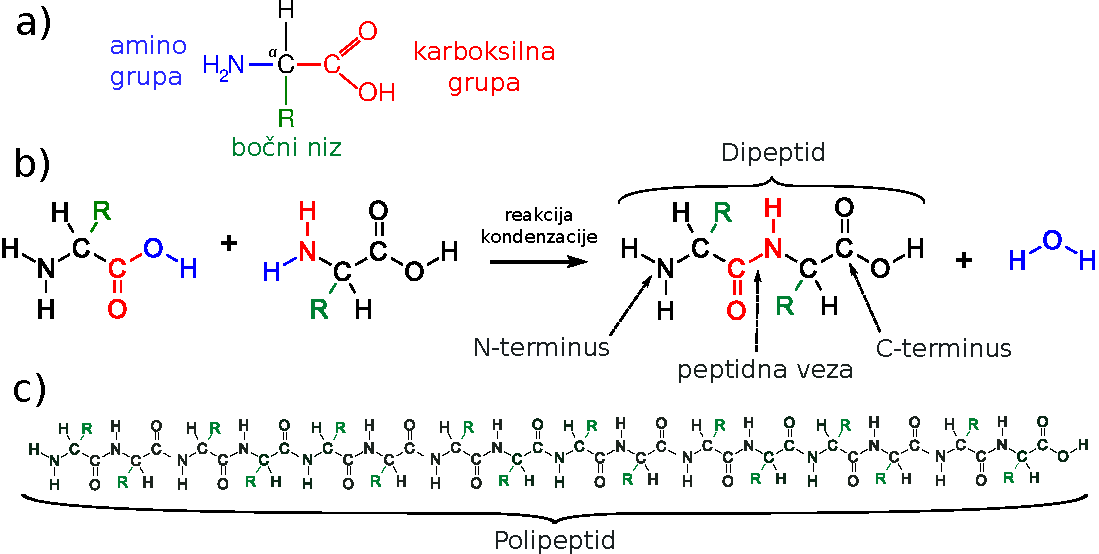
\includegraphics[scale=0.8]{uvod/aminokiselina.pdf}
\caption {a) Šematski prikaz aminokiseline
b) Spajanje aminokiselina reakcijom kondenzacije
c) šematski prikaz polipeptida
}
\label{fig:AK}
\end{figure}


\begin{figure}[th]
\centering
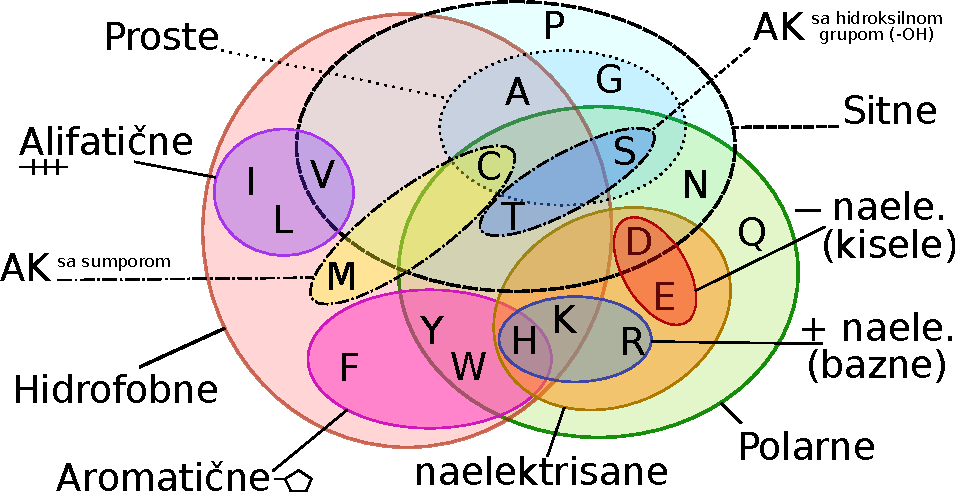
\includegraphics[scale=0.9]{uvod/AK_vene.pdf}
\caption {Veneov dijagram osobina bočnih nizova aminokiselina}
\label{fig:AK_vene}
\end{figure}

\clearpage


\subsection{Struktura proteina}

Protein je sačinjen iz jednog (monomerni) ili više (oligomerni) polipeptidnih lanaca.
Proteinska struktura (oblik) opisuje se kroz četiri nivoa rastuće složenosti.

\keyword{Primarna struktura} opisana je redosledom peptidnih veza kičme peptida,
odnosno redosledom aminokiselina. Primarna struktura predstavlja \keyword{sekvencu
proteina} i kompaktno je zapisujemo azbukom od minimum 20 karaktera.

\keyword{Sekundarna struktura} najčešće nastaje formiranjem vodoničnih veza
između atoma kiseonika i azota istog lanca peptida stvarajući na taj način
dva različita oblika koja su prikazana na Slici \ref{fig:sekundarna}:
\begin{itemize}
  \item \keyword{$\alpha$-spirala} - spiralna struktura u kojoj R grupe štrče spolja
  \item \keyword{$\beta$-traka}  - spoj dva ili više (anti)paralelnih delova polipeptidnog lanca.
\end{itemize}

\begin{figure}[th]
\centering
\hspace*{-2.0cm} 
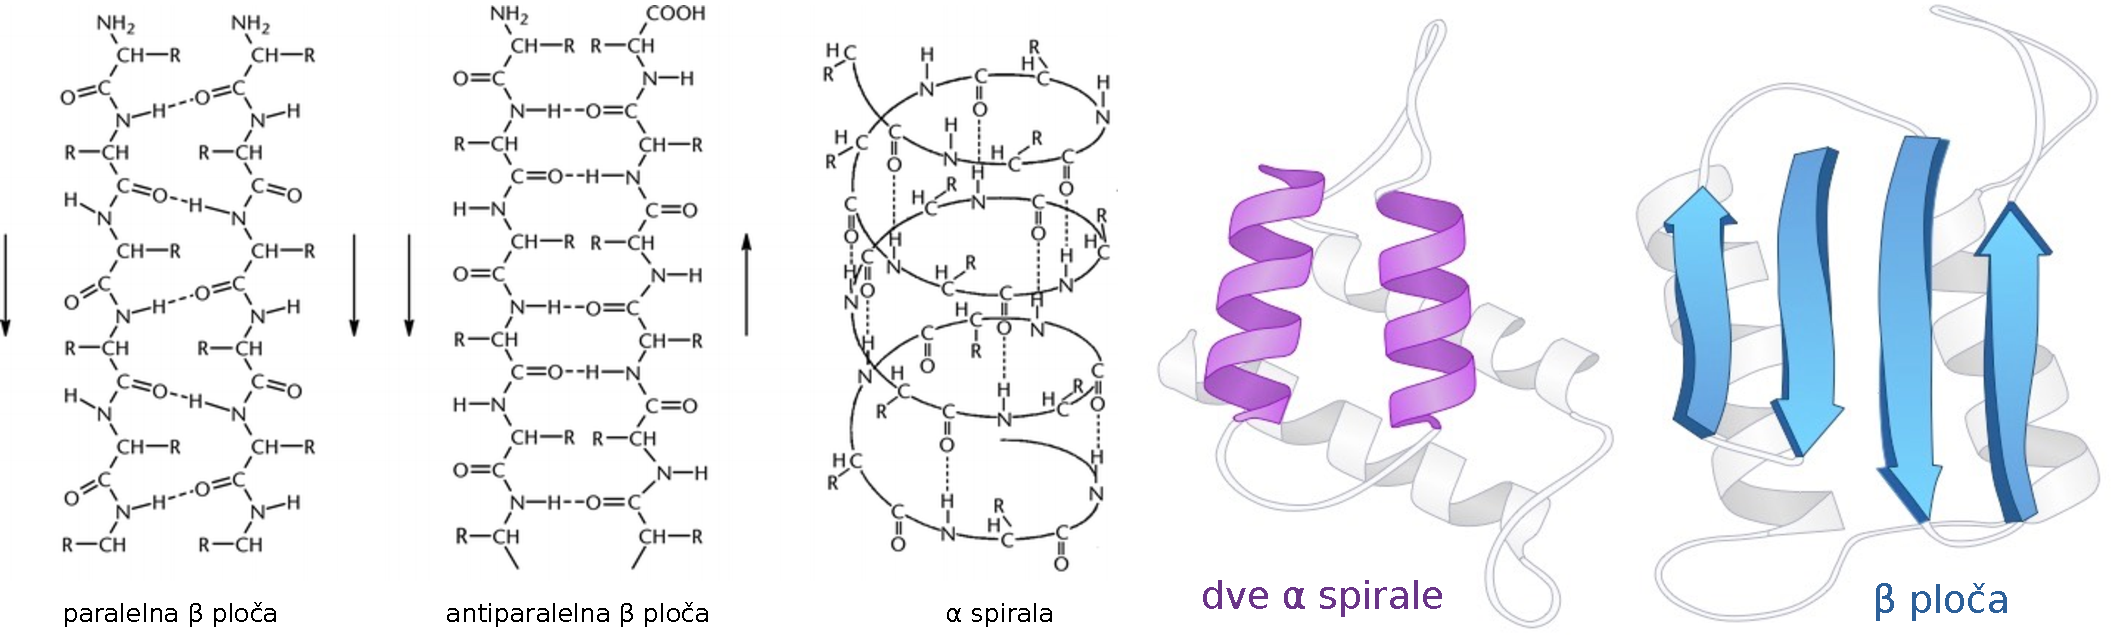
\includegraphics[scale=0.53]{uvod/sekundarna.pdf}
\caption {
  Sekundarna struktura $\alpha$-spirala i $\beta$-traka. \footnotesize Levi deo slike preuzet je sa \parencite{sekundarna_ref_a}.
  Desni deo slike preuzet je sa \parencite{sekundarna_ref_b}.
}
\label{fig:sekundarna}
\end{figure}

Delovi pp lanca  koji povezuju navedene strukture (Slika \ref{fig:sekundarna}b
) često nemaju uređenje i po dužini ih delimo na kraći zaokretaj i duže petlje
\en{short turn, long loop}. Specijalno, $\beta$-ukosnica \en{$\beta$-hairpin} je
kratak zaokret lanca kod antiparalelne $\beta$-trake.  Formiranje sekundarne
strukture naziva se \keyword{lokalno savijanje}.

Usled deljenja elektrona,  peptidna veza ponaša se slično dvostrukoj kovalentnoj
vezi i onemogućava rotaciju ograničavanjem mogućih konformacija pp lanca.
Ovakvo ponašanje dozvoljava kreiranje pravilnih sekundarnih struktura
dodatnim ograničavanjem vrednosti tzv.  dihedralnih uglova $\psi$ i $\phi$ prikazanih
na Slici \ref{fig:uglovi}a. 
Sekundarne strukture ($\alpha$-spirala i $\beta$-traka) imaju specifične kombinacije
vrednosti $\psi$ i $\phi$ uglova. Ove kombinacije ilustrovane su skicom
Ramačandranovog dijagrama (Slika \ref{fig:uglovi}b) koji se dobija kao
šema raspršenih elemenata \en{scatter plot} svih $\psi$ i $\phi$ vrednosti jednog polipeptida.


Pored gore navedenih, disulfidni most\footnote{
  Disulfidni most se formira izvan ćelije, nakon što je protein  već savijen, i
  služi stabilizaciji 3D strukture.
},
cinkovi prsti i ukosnica takođe se smatraju elementima sekundarne strukture.
Postoje i drugi oblici spirala i traka, ali ih nećemo navoditi.




\keyword{Tercijarna struktura} predstavlja prostorni oblik koji protein zauzima
indukovan interakcijama bočnih nizova aminokiselina. Ovaj korak poznat je kao
\keyword{savijanje} \en{folding}.  Pod poznavanjem tercijarne strukture 
podrazumeva se opisivanje prostornih koordinata svih atoma polipeptida. Primer dijagrama
tercijarne strukture dat je Slikom \ref{fig:sekundarna}b.
Najveći uticaj na formiranje sekundarne strukture ima polarnost aminokiselina.
Tercijarna struktura proteina obično je podeljena u jedan ili više
\keyword{domena} koji predstavljaju rigidne savijene regione pp lanca.  Domeni
su obično sačinjeni od nekoliko elemenata sekundarne strukture.

\keyword{ Kvaternerna struktura } opisuje proteinske komplekse (oligomerne proteine) sastavljene
iz nekoliko savijenih polipeptida. Na primer, hemoglobin je proteinski kompleks.

Savijanje proteina u funkcionalan oblik (oblik koji indukuje biološku funkciju)
odnosno njegova tercijarna ili kvaternerna struktura direktno zavise od
primarne strukture tj. sekvence. Dovoljna je zamena jedne aminokiseline u sekvenci
pa da protein izgubi sekundarnu, a time i tercijarnu strukturu gubeći mogućnost
izvršavanja biološke funkcije. Familija proteina obično je okarakterisana
sličnošću domena, pa još kažemo da su domeni \keyword{konzervirani} ili očuvani.
Konzervirani elementi sekundarne strukture domena predstavljaju
\keyword{strukturni motivi}, kraće \keyword{motiv} i okarakterisani su velikom
sličnošću primarne strukture. Promena okruženja (ph, temperature) dovodi do promene
tercijarne strukture ili potpunog gubitka strukture (denaturacija).


\begin{figure}[th]
\centering
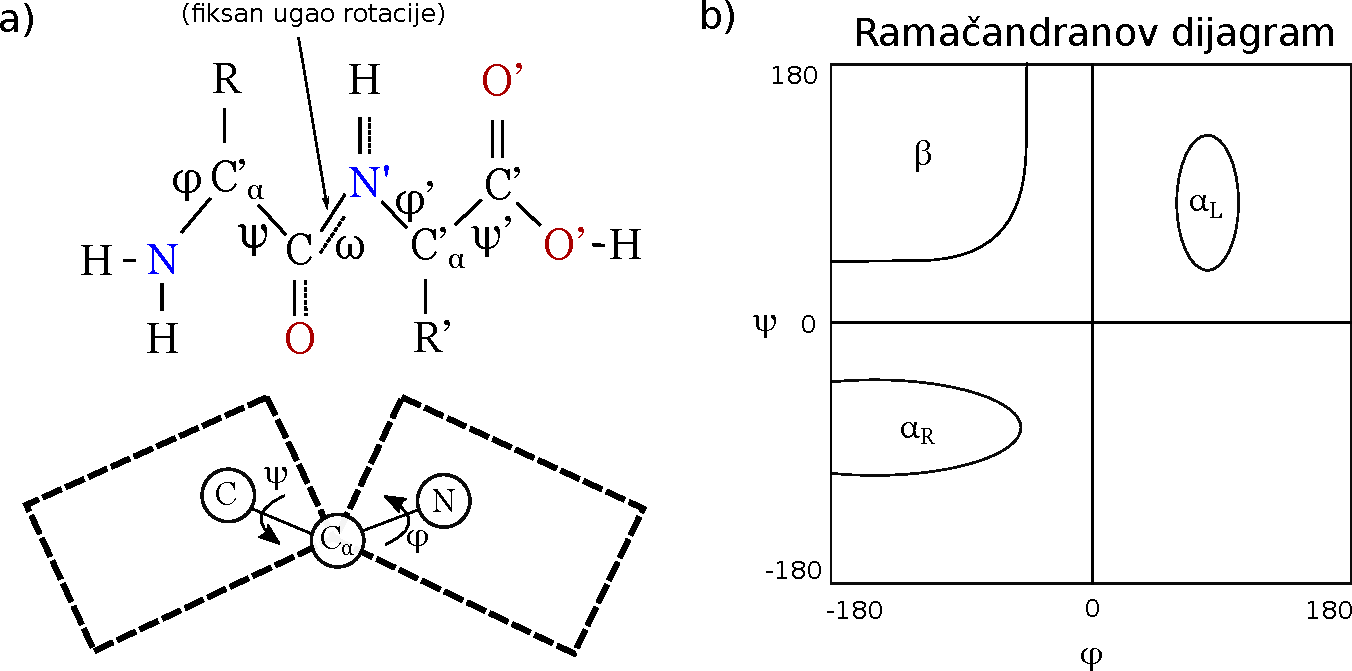
\includegraphics[scale=0.6]{uvod/uglovi.pdf}
\caption {
  \footnotesize
  a) Prikazuje, $\psi$, $\phi$ i $\omega$ uglove. Ugao $\omega$ je fiksan
  zbog specifičnosti peptidne veze omogućavajući rotiacije samo oko
  $\psi$ i $\phi$ uglova.
  b) Skica ramačandranovog dijagram, prikazuje najčešću raspodelu vrednosti uglova
  i sekundarne strukture koje oni obrazuju.
  (Dijagrami su preuzeti iz \cite{Bioinformatics2007})
}
\label{fig:uglovi}
\end{figure}


% Roles:
% Proteini formiraju strukturu (kosa, nokti, perje, colagen)
% proteins effect movments
% Zaštitna uloga (antigeni)
% Transportna uloga, kontrolišu ulazak jona u ćeliju
% Primaju stimulus i transmituju informaciju
% Komunikacija između ćelija (hormoni, većina su proteini, insulin)
% control and regulate processes
% Catalyze chemicall reactions (enzimi)

\subsection{Enzimi}

Život na ćelijskom nivou tj. održavanje balansa (homeostaze) zahteva hemijske
reakcije koje se pri fiziološkim uslovima\footnote{Pod fiziološkim uslovima
podrazumevaju se normalni uslovi u živoj ćeliji (ph, temperatura, ...)} ne
izvršavaju dovoljno brzo ili ne vrše.
\keyword{Katalizator} je molekul koji ubrzava hemijsku reakciju bez da sam bude
promenjen. \keyword{Enzim} je katalizator biološkog porekla, a najčešće je protein.
Molekul koji biva \keyword{katalizovan} odnosno promenjen u interakciji sa
enizmom zovemo \keyword{supstrat}. Mesto enzima koje interaguje sa
supstratom naziva se \keyword{aktivni region}.  Skoro svaka reakcija u živom
organizmu ubrzana je enzimskom katalizom. Ime enzima obično se završava na '-za'
Karakteristika enzima je da katalizuje reakciju specifičnog molekula.

\subsection{Funkcija proteina}

% Udžbenici iz biologije često nabrajaju uloge koje protein ima
Primeri uloga koje protein može da ima uključuju: formiranje
strukture, zaštitna uloga (tzv. antigeni), transport, katalizacija hemijskih
reakcija (enzimi), regulacija procesa u ćeliji itd.  Postoji nekoliko sistema
(nomenklatura) za razdvajanje proteina po funkciji.  Na primer, specijalno za
enzime postoji numerička klasifikacija po hemijskoj reakciji koju katalizuju.
Pomenuta klasifikacija klasteruje enzime u hijerarhiju podskupova. Ovaj pristup
nije adekvatan u opštem slučaju jer skupovi i podskupovi nisu adekvatni za
reprezentaciju ponašanja svih proteina.

\keyword{Ontologija} predstavlja podobniju strukturu koja je oblika acikličkog
usmerenog grafa.  Ontologije su nastale u cilju opisivanja sveta, odnosno
stvari koje ga čine, njihove međusobne relacije i predstavlja oblast
filozofije.  Gore navedena klasifikacija enzima može se predstaviti kao
specijalan slučaj ontologije tj. stablo sa jednim tipom roditeljske veze
(\textit{is\_a} veza).

Protein može biti sagledan iz nekoliko uglova, na primer kom procesu pripada,
gde se taj proces odvija u ćeliji i koja je molekulska funkcija koju obavlja
tokom izvršavanja pomenutog procesa. Sve tri stavke daju uvid u funkciju
proteina i mogu biti predstavljene ontologijama. U ovom radu od interesa je
isključivo molekulska funkcija proteina.  Detaljan opis  molekulske funkcije i
ontologije koja je predstavlja dat je u Poglavlju \ref{GO} i Potpoglavlju
\ref{MF}.




% Roles:
% Proteini formiraju strukturu (kosa, nokti, perje, colagen)
% proteins effect movments
% Zaštitna uloga (antigeni)
% Transportna uloga, kontrolišu ulazak jona u ćeliju
% Primaju stimulus i transmituju informaciju
% Komunikacija između ćelija (hormoni, većina su proteini, insulin)
% control and regulate processes
% Catalyze chemicall reactions (enzimi)

% Dopisati

% \textit{
% Ovde govorimo o funkciji proteina uopste. Prikladnije je prvo objasniti da je
% najcesci nacin predstavljanja funkcija preko GO ontologija, a onda navesti i
% isecak iz GO ontologije
% Tabelu 2.1 koja je iz rada navesti kasnije kada budemo govorili o metodama i
% podacima. 
% Ne navodimo da se nadamo da cemo potvrditi, iako to zaista jeste tako. Mozemo
% navesti da ispitujemo da li nesto vazi ali nije praksa eksplicitno pisati da se
% nadamo da nesto vazi
% }


% Funkcija proteina može biti sagledana iz tri ugla: molekulske funkcije,
% biološkog procesa kome pripada i lokacije u ćeliji gde se funkcija odvija
% \parencite{go2000}(postoje i drugi sistemi klasifikacije\ref{keyword}).  Kako
% je cilj ovog rada molekulska funkcija Tabelom\ref{tab:funkcija_uvod} ukratko
% navodimo (bez poretka) ustanovljene \parencite{Xie2007} molekulske funkcije koje
% se pripisuju (ne)uređenosti proteina. Ovo su takođe rezultati za koje se nadamo
% da će naše istraživanje potvrditi.
%
% \begin{table}[h!]
%   \centering
%   \caption{Odnos molekulske funkcije i uređenosti}
%   \label{tab:funkcija_uvod}
%   \begin{tabular}{c}
%   
%   \end{tabular}
% \end{table}
%
%
%
% \keyword{Ovo možda za kraj ostaviti...} \\
% Novija istraživanja nad eksperimentalno dokazanih IDP i IDPr dovela su do
% kreiranja ontologija(po ugledu na GO \parencite{GO2000}) za opis funkcija
% neuređenih proteina. Ontologije su sastavni deo DisProt \parencite{disprot7}
% baze eksperimentalno dokazanih IDP i IDPr... novi prediktori postoje...



% \subsection{Teorija informacija}
%
%
% \subsection{Ontologije i funkcija}
